% ============================================================
\chapter{Design Considerations}
% ============================================================

\section{Design Constraints}

Beyond the functional and non-functional requirements set out in Chapter~3,
three further constraints shaped how NetMind was designed: the hardware and
software environment the team actually had available, the characteristics of
the people the system is meant to serve, and the single academic term within
which a working system had to be built and demonstrated.

\subsection{Hardware and Software Environment}

NetMind had to run comfortably on each team member's own laptop rather than
on dedicated lab or cloud hardware, which ruled out heavier,
virtual-machine-based network emulators in favour of a lightweight,
container-based one. The simulated network alone comprises a core router,
three branch firewalls, three switch/hub segments, eight hosts, and three
cameras (eighteen nodes in total: fifteen containers and three bridge
segments), so the chosen tooling had to start, stop, and be queried quickly
without exhausting a single machine's resources. Because Docker Desktop's
bundled engine does not reliably expose the Linux network-namespace and
bridge access that Containerlab needs to wire virtual links between
containers, the team standardised on a native docker-ce engine running inside
a WSL2 Ubuntu distribution on each member's Windows machine, with
Containerlab itself used only once per deployment to build the topology from
a declarative YAML file. Figure~\ref{fig:environment} shows how the pieces of
this environment fit together, from the browser-based application down to
the simulated network itself and out to the external language-model
provider. Table~\ref{tab:environment} summarises the specific components of
this environment and the role each one plays.

\begin{figure}[H]
\centering
\begin{tikzpicture}[
  font=\small,
  box/.style={draw,rounded corners=2pt,fill=boxgray,align=center,inner sep=4pt},
  cloud/.style={box,fill=white},
  zl/.style={font=\scriptsize\itshape,anchor=north west,inner sep=2pt},
  note/.style={font=\scriptsize\itshape},
  >={Stealth[length=2.2mm]}]
  % zones (drawn first, explicit coordinates)
  \draw[dashed] (-0.3,0.3) rectangle (9.0,-6.9);
  \node[zl] at (-0.3,0.3) {Team member's laptop (Windows host)};
  \draw[dashed] (0.0,-2.0) rectangle (8.7,-6.6);
  \node[zl] at (0.0,-2.0) {WSL2 Ubuntu};
  \draw[dashed] (3.4,-4.6) rectangle (8.4,-6.35);
  \node[zl,anchor=north east] at (8.4,-4.6) {native docker-ce engine};
  % boxes
  \node[box,text width=5.4cm] (browser) at (4.35,-0.95)
    {\textbf{Browser}\\chat, dashboard, alerts, logs,\\reports, confirm box (EN/AR)};
  \node[box,text width=5.0cm] (api) at (4.35,-3.2)
    {\textbf{FastAPI backend} (\code{web\_server.py})\\agent loop, safety guard, tool registry};
  \node[box,text width=2.3cm] (db) at (1.6,-5.55) {\textbf{SQLite}\\sessions,\\audit log};
  \node[box,text width=4.4cm] (lab) at (5.9,-5.55)
    {\textbf{Containerlab topology}\\1 router, 3 firewalls,\\3 switch/hub segments,\\8 hosts, 3 cameras};
  \node[cloud,text width=3.0cm] (groq) at (11.6,-3.2) {\textbf{Groq cloud API}\\\code{gpt-oss-120b}};
  \node[cloud,text width=3.0cm] (tg) at (11.6,-5.55) {\textbf{Telegram}\\alert notifications};
  % arrows
  \draw[<->] (browser) -- node[right,note,pos=0.72]{REST, 127.0.0.1 only} (api);
  \draw[->] (api) -- node[above,note,pos=0.75]{tool calls} (groq);
  \draw[->,dashed] ([yshift=-3mm]api.east) -| (9.6,-5.55) -- (tg.west);
  \draw[->] ([xshift=-1.6cm]api.south) |- ++(0,-0.5) -| (db.north);
  \draw[->] ([xshift=1.4cm]api.south) -- node[left,note,pos=0.4]{Docker SDK} ([xshift=1.4cm]api.south |- lab.north);
\end{tikzpicture}
\caption{NetMind development and deployment environment}
\label{fig:environment}
\end{figure}

{\small
\begin{xltabular}{\textwidth}{|L{3.4cm}|Y|}
\hline
\head \textbf{Component} & \textbf{Role} \\ \hline
\endhead
Host OS & Windows 10/11 laptop belonging to each team member, running a WSL2 Ubuntu distribution \\ \hline
Container runtime & Native docker-ce engine inside WSL2 (not Docker Desktop's own engine) \\ \hline
Network emulation & Containerlab, used once per deployment to build the topology from a YAML file \\ \hline
Router node & FRRouting (\code{frrouting/frr}) image acting as the core router \\ \hline
Firewall nodes & Custom Alpine-based image running live iptables rules \\ \hline
Camera nodes & Custom Alpine-based image running a small Python HTTP service \\ \hline
Backend & Python 3 / FastAPI, communicating with Docker through the Docker SDK \\ \hline
Storage & SQLite (Python standard library) for chat sessions and the audit log; a JSON file for the alert history \\ \hline
Frontend & Vanilla JavaScript single-page application with chat, live dashboard, devices, alerts, logs and reports views, an in-page confirmation box, English/Arabic and light/dark themes, no build step \\ \hline
Language model & Groq API, \code{openai/gpt-oss-120b}, via an OpenAI-compatible tool-calling interface behind a provider interface \\ \hline
Notifications & Telegram Bot API (optional) for alerts outside the browser \\ \hline
Version control & Git, hosted on GitHub, with one issue per task and all changes merged by pull request \\ \hline
Continuous integration & GitHub Actions workflow running ruff and pytest, with a minimum test coverage, on every pull request \\ \hline
Lab automation & Makefile (\code{make up}, \code{make down}, \code{make run}, \code{make test}, \code{make lint}, \code{make setup-perms}) with idempotent bridge creation \\ \hline
\caption{Development and deployment environment}\label{tab:environment}\\
\end{xltabular}}

\subsection{End User Characteristics}

As set out in Chapter~3, NetMind is designed for an operator of a small or
medium branch network who may not be a dedicated network engineer: someone
comfortable with basic networking concepts such as an IP address or a
firewall port, but not necessarily fluent in any single vendor's command-line
syntax. Because the development team and the project's academic context are
Arabic-and-English bilingual, the same assumption was extended to language: a
user should be able to work entirely in whichever of the two languages they
are more comfortable in, without the system defaulting to one over the other.
Table~\ref{tab:users} summarises the characteristics assumed of this end user
and the design decision each one led to.

{\small
\begin{xltabular}{\textwidth}{|Y|Y|}
\hline
\head \textbf{Characteristic} & \textbf{Design Implication} \\ \hline
\endhead
Not a dedicated network engineer & Natural-language chat interface rather than a command-line or vendor-specific console (NFR1) \\ \hline
Comfortable in Arabic or English, not necessarily both equally & Bilingual input and output, matching the language of each request (NFR2) \\ \hline
Accesses the system from a standard laptop browser & No client installation; browser-only frontend (NFR13) \\ \hline
Expects a quick answer, not a slow diagnostic tool & Low-latency LLM provider and a bounded tool-calling loop (NFR9, NFR10) \\ \hline
May need to tell Simulated and Real Network mode apart at a glance & An always-visible control distinguishing the two modes (NFR3) \\ \hline
Responsible for device security, not just connectivity & Firewall auditing and camera credential checks exposed as first-class capabilities (FR4, FR6) \\ \hline
Is not always looking at the screen & Alerts kept as a history and sent to Telegram (FR10, FR15) \\ \hline
\caption{End-user characteristics and their design implications}\label{tab:users}\\
\end{xltabular}}

\section{Architectural Strategies}

\subsection{Development Method}

NetMind was built using an iterative, prototype-first method rather than a
single upfront design, an approach the supervisor, Dr.\ Khalil Chebil,
actively encouraged given the project's one-term timeline and its dependence
on infrastructure (the simulated network) that could only really be validated
once it existed. Each capability was built as a self-contained increment:
device status and power control first, then firewall auditing, then camera
security, and finally real-network discovery. Each increment was deployed
against the live Containerlab lab and reviewed with the supervisor before the
next one began, rather than being designed in isolation from working
infrastructure. Figure~\ref{fig:method} illustrates this loop.

\begin{figure}[H]
\centering
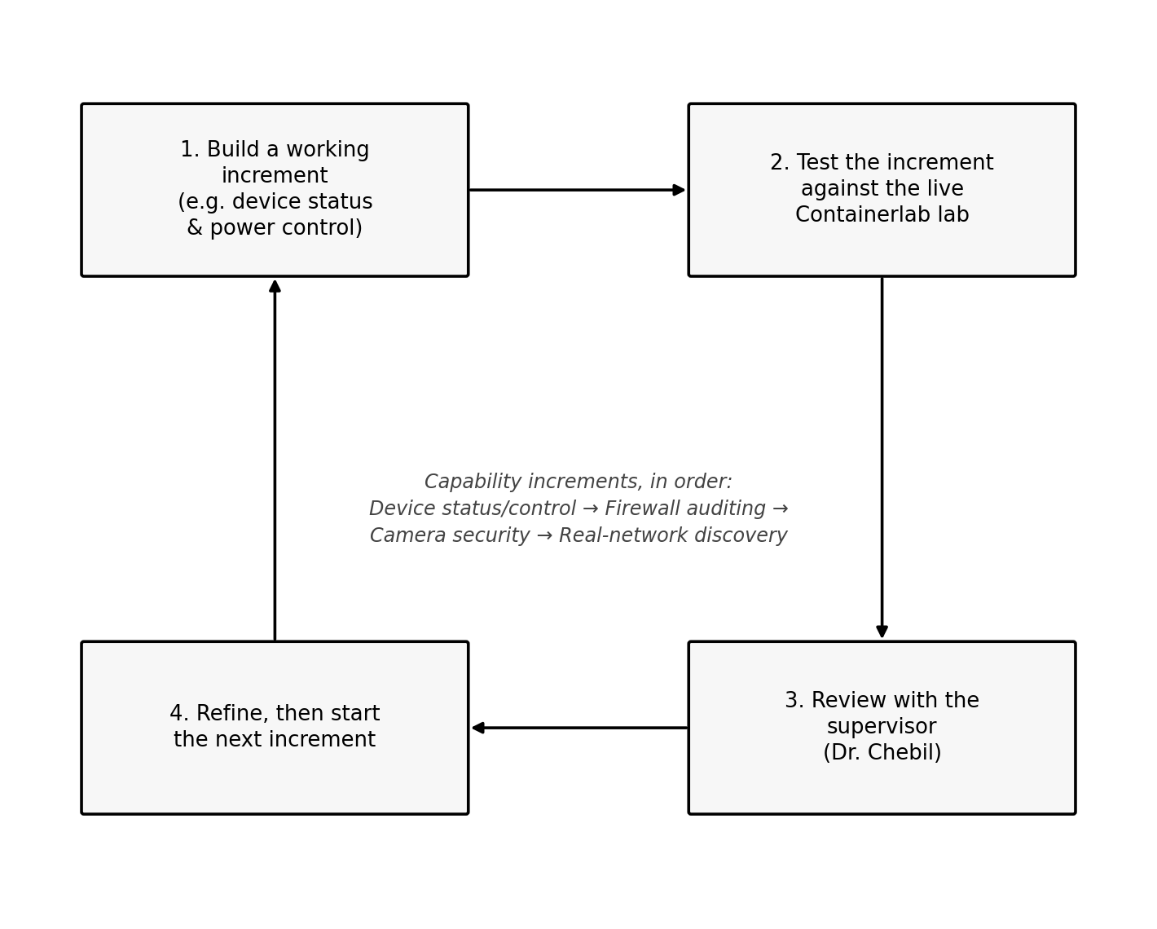
\includegraphics[width=0.72\textwidth]{dev-method.png}
\caption{Iterative, supervisor-reviewed development method}
\label{fig:method}
\end{figure}

This incremental approach meant that a demonstrable, working system existed
from early in the project, and that any gaps a given increment left behind
were identified against a real, running lab rather than assumed away on
paper. At the end of September the supervisor reviewed the whole system and
prepared an assessment and a seven-month improvement plan (October 2026 to
April 2027) organised as monthly milestones. From October onwards the team
therefore worked from that plan: every task became a GitHub issue, every
change was made on its own branch and merged through a pull request that
needed the continuous-integration checks to pass, and the work was split
across three tracks (core backend, AI agent, and frontend and real network)
so that each member has individually assessable contributions. The first two
milestones, stabilisation (October) and the architecture refactor
(November), are complete.

\subsection{Future Enhancements and Plans}

The current system intentionally leaves work for Project 2. The supervisor's
plan sets out the remaining milestones, and the team has added two items of
its own that build directly on the existing tool registry and agent loop.
Table~\ref{tab:p2plan} outlines the main areas; Section~6.3 lists them in
more detail.

{\small
\begin{xltabular}{\textwidth}{|L{3.2cm}|Y|}
\hline
\head \textbf{Area} & \textbf{Planned Enhancement} \\ \hline
\endhead
Observability & A background collector with a per-device state machine, so alerts are raised even when nobody has the dashboard open; diagnostic and alert-history tools for the agent \\ \hline
Diagnosis & Reversible fault-injection scenarios and root-cause-analysis playbooks that diagnose a fault with evidence \\ \hline
Safe change & Proactive fix suggestions, firewall snapshots with diff and rollback, and authentication with roles (NFR7) \\ \hline
Evaluation & A benchmark of 100+ English and Arabic prompts, a comparison of LLM providers and models, load testing, and a usability study \\ \hline
Integration & An MCP server exposing NetMind's tools to other AI assistants, and a hardened agent harness \\ \hline
\caption{Planned enhancements for Project 2}\label{tab:p2plan}\\
\end{xltabular}}
